 \chapter{EOM Combs}

In this chapter, I discuss the generation of high-repetition-rate frequency combs through electro-optic modulation of a continuous-wave laser – so-called EOM combs \cite{Kobayashi1972,Kourogi1993,Murata2000,Sakamoto2007,Morohashi2008,Ishizawa2010,Wu2010,Supradeepa2012,Metcalf2013,Wu2013}. This scheme represents an alternative to parametric generation of HRR combs in Kerr resonators, and as the technology matures it will likely find a niche in the application space that leverages its long-term stability, lack of moving parts, and possibility for robust turn-key operation. First I present the operational principle, and then experimental results that represent the first generation of a coherent octave-spanning supercontinuum and detection of an active-modulation-based frequency comb's carrier-envelope offset frequency without an external optical reference. Then I provide a detailed discussion of the noise properties of the EOM comb, the investigation of which is a significant contribution of the work described here. Finally, I provide a discussion of some possible future directions for the technology.

\section{Principle of operation}
Generally, the EOM comb concept consists of passing a CW 'seed' laser through cascaded phase and intensity modulators to generate a train of chirped pulses, and then propagating this pulse train through a dispersive medium to temporally compress the pulses to near their bandwidth-limited pulse duration. An generic expression for the electric field before temporal compression results from the product of the field $E_oe^{-i\omega_ct}$ with operators
\begin{align} \frac{1}{2}\left\{\mathrm{exp}\left[i(\phi_{DC}+\phi_{RF}\sin{\omega_rt})\right]+\mathrm{exp}\left[-i(\phi_{DC}+\phi_{RF}\sin{\omega_rt})\right]\right\}\\
=\cos\left(\phi_{DC}+\phi_{RF} \sin(\omega_rt+\phi_{IM-PM})\right)
\end{align} representing the intensity modulation and 
\begin{equation}
\mathrm{exp}\left[i\beta_m \sin{\omega_r t}\right]
\end{equation} representing the phase modulation. Here $E_o$ and $\omega_c$ are the complex amplitude and the carrier frequency of the seed laser. The phases  $\phi_{DC}$ and $\phi_{RF}$ represent the DC bias and depth of the intensity modulation, respectively, which experimentally are sourced from a DC power supply and an RF synthesizer. Writing the intensity-modulation operator as the sum of exponentials reveals the physical origin of intensity modulation as phase modulation in two paths with opposite sign. The phase-modulation index, which sets the initial bandwidth of the EOM comb, is $\beta_m$. The comb's repetition rate is $f_r=\omega_r/2\pi$, with $\omega_r$ the angular frequency of the phase and intensity modulation, which in practice are derived from the same synthesizer. The phase $\phi_{IM-PM}$ represents a phase difference between the IM and PM operators arising from path-length differences, which can be controlled via the insertion of a phase shifter in one electrical path. 

In practice, for subsequent spectral broadening of the comb it is desirable to configure the IM and PM to yield a train of 50 $\%$ duty-cycle pulses with normal chirp (temporally increasing carrier frequency). To achieve this, both $\phi_{DC}$ and $\phi_{RF}$ are set to $\pi/4$ and $\phi_{IM-PM}$ is set to zero. To achieve the former, the DC bias voltage and the RF modulation amplitude are adjusted to yield the appropriate optical spectrum for the seed laser with only intensity modulation applied. Setting $\phi_{IM-PM}$ to either zero or $\pi$ is achieved by examining the optical spectrum of the EOM comb with both IM and PM applied. The spectrum is asymmetric if $\phi_{IM-PM}$ is not zero or $\pi$ due to stronger transmission of either the high- or low-frequency components of the phase-modulated seed laser through the intensity modulators. The optical spectrum of the comb, which does not include phase information, is the same for $\phi_{IM-PM}=0$ or $\pi$; the difference between the two corresponds to reversal of the field in time or, equivalently, the difference between normal and anomalous chirp. In practice, setting $\phi_{IM-PM}$ to zero can be achieved by verifying that the pulses are compressed by propagation in an appropriate length of an anomalously dispersive medium; $\phi_{IM-PM}=\pi$ corresponds to anomalous chirp.

A simplified and illuminating expression for the electric field of a normally-chirped 50 $\%$ duty-cycle pulse train (up to a constant overall phase shift relative to the previous expression) is:
\begin{equation}
E=E_o\cos\left(\frac{\pi}{2}\sin^2{\frac{\omega_rt}{2}}\right)e^{i\omega_ct-i\beta_m\cos{\omega_rt}}.
\end{equation}
This can be understood as the product of a time-varying real amplitude $a(t)=E_o\cos\left(\frac{\pi}{2}\sin^2{\frac{\omega_rt}{2}}\right)$ and a phase factor from which the instantaneous carrier frequency $\omega(t)=\omega_c+\omega_r\beta_m\sin{\omega_rt}$ can be calculated. The carrier frequency $\omega(t)$ is increasing when the amplitude $a(t)$ is at its maximum, corresponding to normal chirp on the pulses.


\section{Detection of the carrier-envelope offset frequency of an EOM comb}

Here I describe generation of an EOM comb with 10 GHz repetition rate and subsequent measurement of its carrier-envelope offset frequency. The experimental setup is depicted in Fig. 1a. The basic experimental scheme consists of the following steps: 1. Initial generation and temporal compression of the EOM comb pulse train; 2. Modest spectral broadening and temporal re-compression; 3. Noise reduction using a Fabry-Perot filter cavity; and 4. Octave-spanning supercontinuum generation and detection of the carrier-envelope offset frequency. The results described below represent the first time a frequency comb based on active modulation of a CW laser has been self-referenced. Key to the success of this approach is the implementation of nonlinear spectral broadening in two stages, which allows the second stage to be seeded with $\sim$130 fs pulses for coherent supercontinuum generation. The noise reduction stage is also critical for coherent spectral broadening, and the investigation of its effects is a significant contribution of this work. 

To generate the initial train of chirped pulses, a telecom-band continuous-wave laser is passed through cascaded phase and intensity modulators driven with a 10 GHz microwave signal. The intensity modulator is biased at the 50 \% transmission point and driven with an RF amplitude appropriate for generation of a 50 $\%$ duty-cycle pulse train, as described above.   The phase modulator is driven with modulation depth of $\sim31\pi/4\sim24.3$ rad. The relative phase between the modulators is set such that the phase applied by the phase modulator is at a minimum when the transmission of the intensity modulator is highest; this yields a train of normally-chirped (up-chirped) pulses. Simulated temporal intensity and instantaneous carrier-frequency profiles are shown in Fig. 1b, and a simulated optical spectrum is overlaid on an experimental measurement in Fig. 1c.


\begin{figure}[htpb]
	\begin{center}
		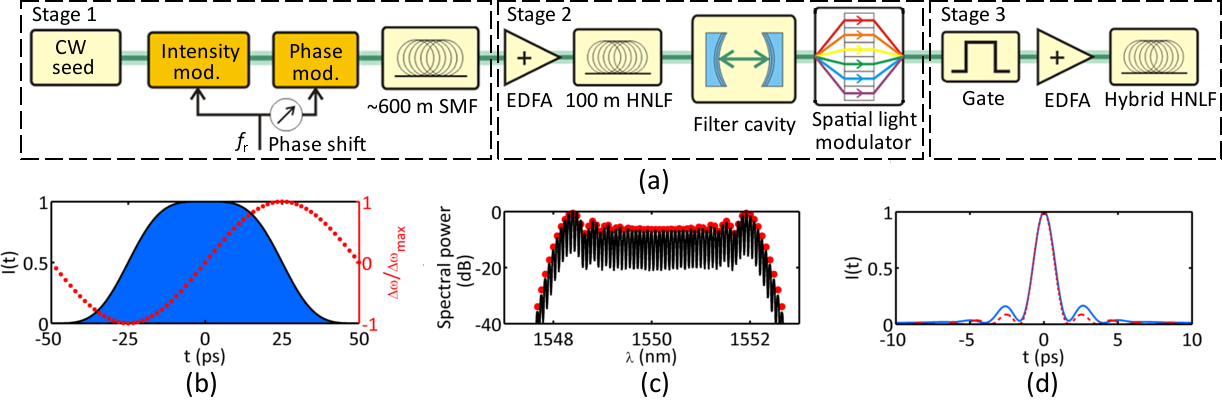
\includegraphics[width=15cm]{\FigPath/Figures/EOMCombs/EOMCSchematic.png}
	\end{center}
	\caption[Figure Title]{\textbf{Schematic and principle of operation for detection of the carrier-envelope offset frqeuency of an EOM comb.} (a) Experimental schematic for $f_0$ detection, with three stages: 1. Initial generation and temporal compression of the pulse train; 2. First stage of spectral broadening and temporal re-compression, along with noise suppression, and 3. Final stage of spectral broadening for generation of a coherent octave-spanning supercontinuum, including the implementation of an electro-optic gate for repetition-rate downsampling. (b) Depiction of a constituent pulse from a train of 50 $\%$ duty-cycle normally-chirped pulses with 10 GHz repetition rate. Intensity is shown in blue, and instantaneous carrier frequency is shown in red. The periodic electric field of this pulse train is given by Eqn. \ref{Eqn:EOMC} (c) Measured optical spectrum of the initial EOM comb pulse train (black), along with the simulated spectrum corresponding to the plots in panel (b). (c) Simulated temporal compression of the pulses shown in panel (b), with compression conducted by propagation in 570 m of SMF (solid blue) and compression to the transform limit (dashed red). The full-width at half-maximum (FWHM) duration of both pulses is $\sim$1.5 ps.   }
	\label{fig:EOMC_Schematic}
\end{figure} 


Next, the chirped pulse train is propagated through 600 m of anomalously-dispersive SMF. The length of SMF that is appropriate for pulse compression depends on the bandwidth of the optical pulses to be compressed; equivalently, it depends on both the phase-modulation depth and the repetition rate of the pulse train. This temporal compression reduces the duration of the optical pulses from $\sim$50 ps to $\sim$ 1.5 ps. A simulation of the resulting intensity profile is presented in Fig. 1d. 

The compressed pulses are amplified to 400 mW average power in an erbium-doped fiber amplifier and launched into 100 m of HNLF. This section of HNLF has chromatic dispersion that is small and normal; this is carefully chosen to chirp the pulses via self-phase modulation while avoiding soliton-fission dynamics\cite{Dudley2006}. The result is a train of chirped $\sim$1.5 ps pulses exiting the fiber.  In Fig. 2a we present the measured optical spectrum of this pulse train, as well as results of a numerical simulation of the spectral broadening in the 100 m of normally-dispersive HNLF. These simulations are conducted using the nonlinear Schrodinger equation (NLSE) including third order dispersion\cite{Agrawal2007}, taking as initial conditions the calculated intensity profile of the EOM comb pulses shown in Fig. 1d. The dispersion values for the HNLF used in the simulation are $D=-0.04$  ps/nm$\cdot$km and $D'=0.003$ ps/nm$^2\cdot$km, close to the values specified by the manufacturer. The simulation method is described in detail in App. \ref{NumericalSims}.

After propagation through the first section of HNLF, the pulses are passed through a high-finesse Fabry-Perot cavity for suppression of optical frequency fluctuations as discussed below. Then the pulses are temporally compressed again, this time using a commercial spatial light modulator (SLM) \cite{Weiner2000}; the SLM separates narrow spectral regions using a grating and passes them through individually controlled delaying elements before recombination. The SLM applies 2\textsuperscript{nd}, 3\textsuperscript{rd}, and 4\textsuperscript{th} order chromatic dispersion, which simulations indicate is sufficient to compress the chirped pulses to $\sim$130 fs, near their transform limit. This is shown in Fig. 2b. While it is convenient, the SLM is not strictly necessary; it would also be possible to compress the pulses via propagation in an appropriate length of SMF. Figs. 2b and 2c present the output intensity profile and the evolution of the intensity profile, respectively, in simulated compression in SMF. Because the pulses are broadband, temporally short, and reasonably high energy, these simulations include the full dispersion profile of SMF and the Kerr nonlinearity.



The temporally compressed $\sim$130 fs pulses are then passed through a Mach-Zehnder modulator functioning as an electro-optic gate for repetition-rate downsampling (see Chapter \ref{PulsePicking}). The gate selectively transmits every fourth pulse, reducing the repetition rate of the pulse train to 2.5 GHz. This facilitates coherent supercontinuum generation in a second stage of spectral broadening by increasing the pulse energy that can be achieved at a given average power. Note that this step is convenient but not strictly necessary, as shown in Ref. \cite{Beha2017}. 

The downsampled 2.5 GHz pulse train is amplified to an average power of 1.4 W, resulting in a train of $\sim$0.56 nJ pulses. This pulse train is propagated through 8 m of hybrid HNLF, yielding the spectrum shown in Fig. 2d. This hybrid HNLF consists of two segments with different dispersion profiles, with each segment serving a different purpose. The first segment is 30 cm long and highly dispersive ($D=6$  ps/nm$\cdot$km), and generates a dispersive wave centered at 1090 nm. The second segment is 7.7 m long and has lower dispersion ($D=1.5$  ps/nm$\cdot$km), and generates a Raman-self-frequency-shifted soliton centered near 2150 nm. The effect of each of these fibers on the output spectrum can be understood by investigating propagation in each section separately. To do this we use the LaserFOAM program \cite{Amorim2009}, which employs the generalized NLSE including Raman scattering, self-steepening, and 2nd- through 4th-order dispersion. The simulations are run independently, and both take as their initial conditions 170 fs Gaussian pulses with 350 pJ energy, close to the energy coupled into the HNLF after accounting for losses. The results of these simulations are plotted in Fig. 2d. 

 % % % % % PulsePickedTrains]
\begin{figure}[htpb]
	\begin{center}
		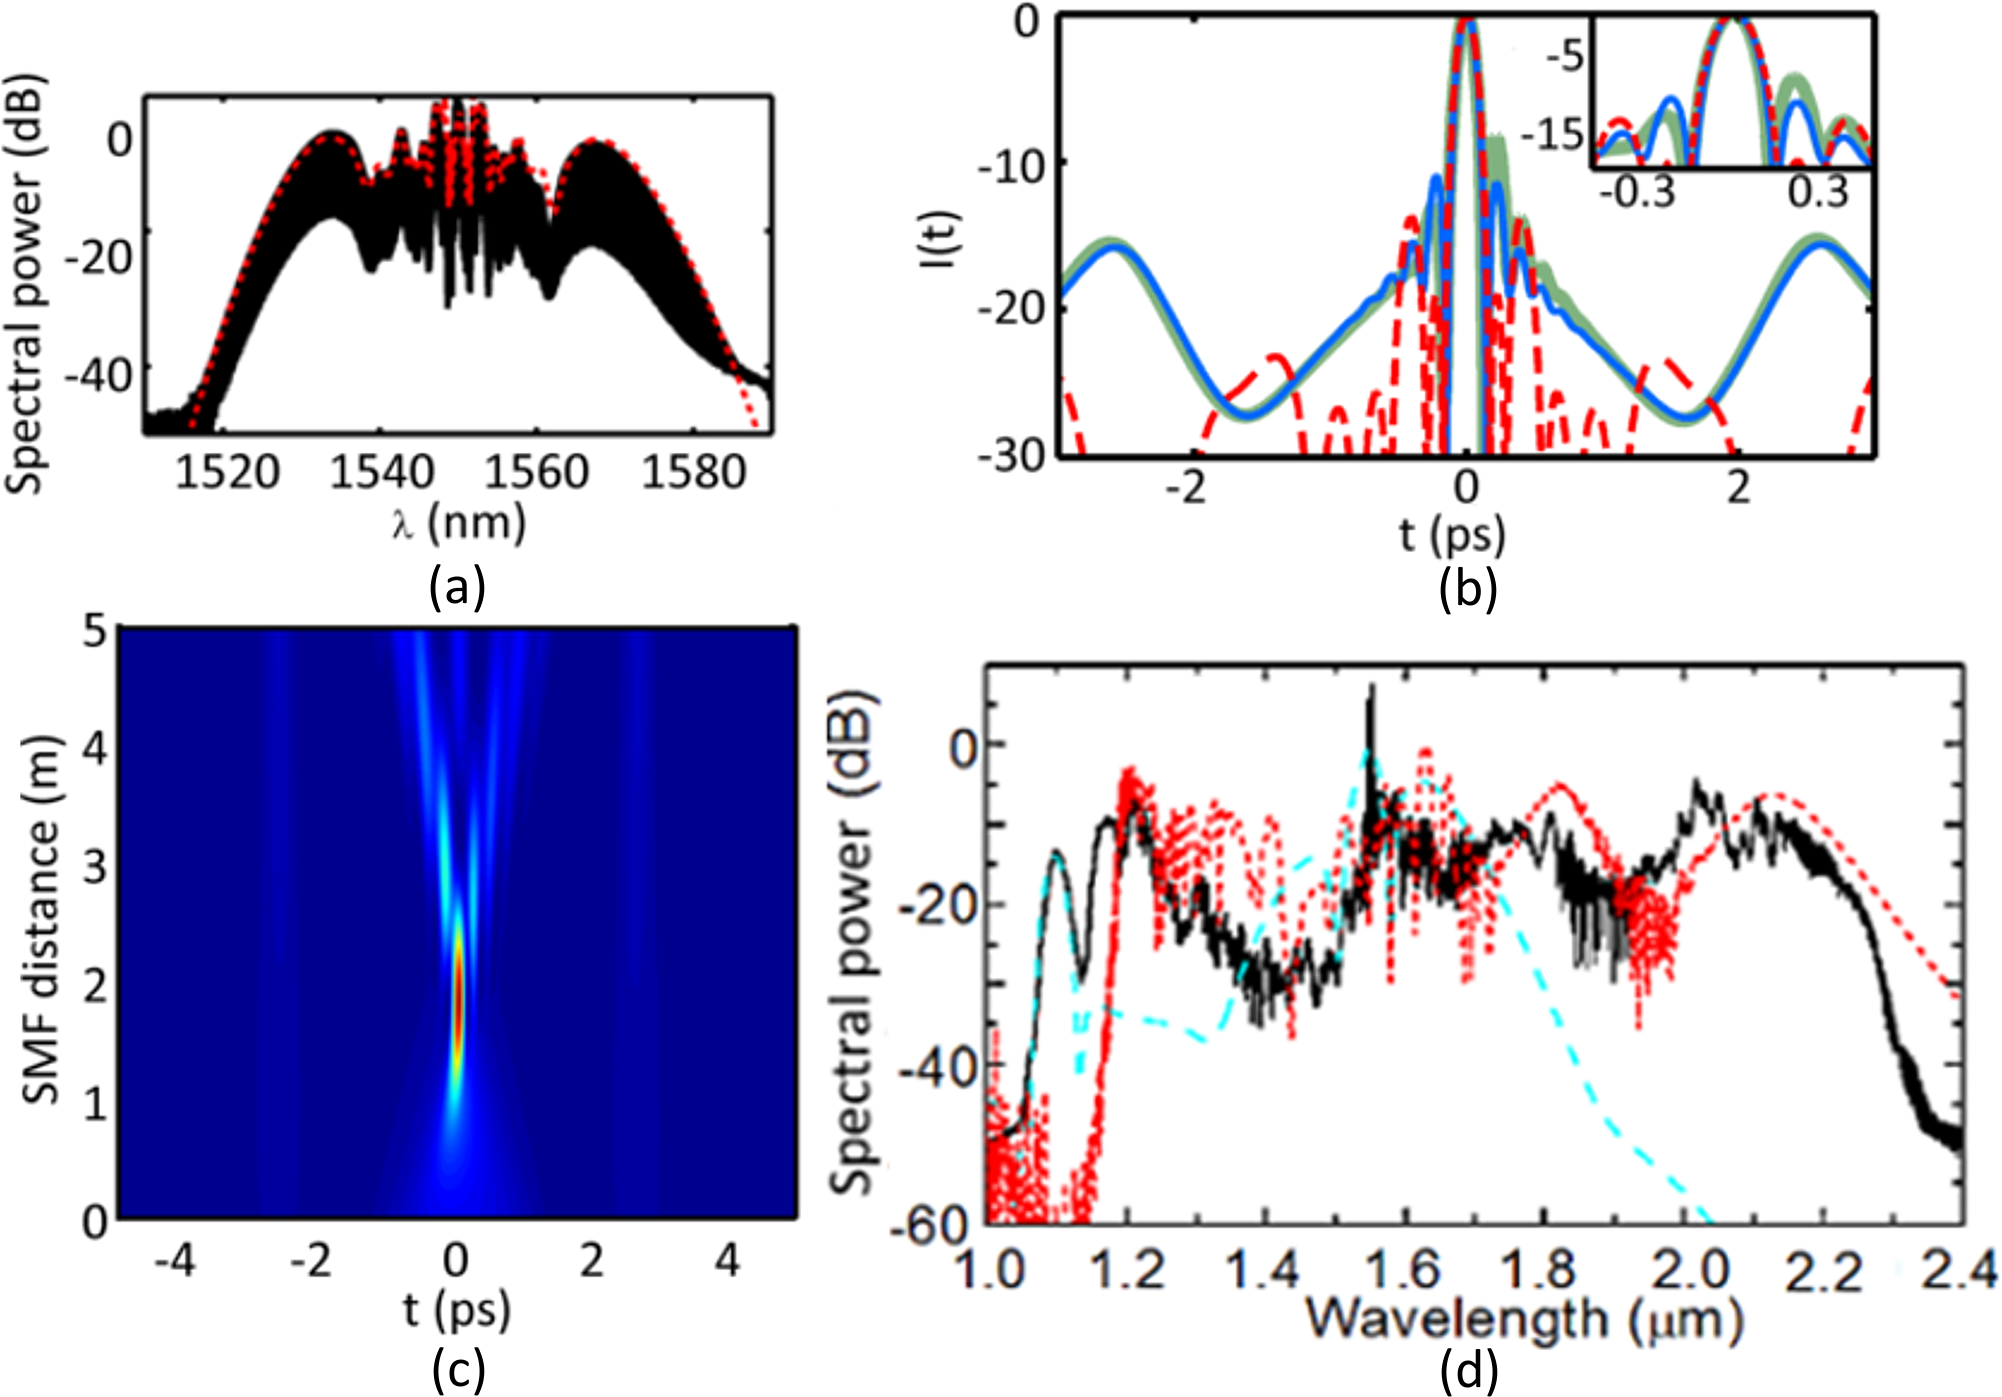
\includegraphics{\FigPath/Figures/EOMCombs/EOMC_spectraWsims.png}
	\end{center}
	\caption[Figure Title]{\textbf{Spectral broadening for generation of an octave-spanning supercontinuum.} (a) Measured optical spectrum after propagation in 100 m of low-normal-dispersion HNLF (black). The spectrum is broadened by self-phase modulation, which imposes a chirp on the pulses. Shown in red is a simulation of the same, conducted as described in the text. (b) Logarithmic-scale plot of the simulated pulse intensity envelopes after temporal recompression in the SLM with 2\textsuperscript{nd}-, 3\textsuperscript{rd}-, and 4\textsuperscript{th}-order dispersion (blue), in an appropriate length of SMF (thick green), to the transform limit (dashed red). (c) Simulated re-compression of the SPM-chirped pulses (red spectrum in panel (a)) in SMF. (d) Measured optical spectrum of the octave-spanning supercontinuum generated by the EOM comb system (black), plotted along with simulated spectra calculated as described in the text to investigate the effects of the 30 cm, highly-dispersive piece of HNLF (long-dashed teal) and the 7.7 m, lower-dispersion piece of HNLF (short-dashed red).}
	\label{fig:EOMC_Broadening}
\end{figure} 

The supercontinuum generated in the hybrid HNLF is coherent and suitable for $f-2f$ self-referencing (see App. \ref{App:f-2f}). To detect the carrier-envelope offset frequency of the EOM comb, we pass the pulse train through an interferometer consisting of a dichroic mirror, a delay stage in one path, and a 10 mm sample of periodically-poled lithium niobate that generates the second harmonic of supercontinuum light at 2140 nm.  The dichroic mirror and delay stage enable adjustment of the relative timing between the native 1070 nm and doubled 2140 nm components of the supercontinuum so that they are temporally coincident. An optical band-pass filter centered at 1070 nm selects the supercontinuum components required for self-referencing, shown in Fig. 3a, and impinging the filtered light on a photodetector reveals the carrier-envelope offset frequency of the EOM comb, shown in Fig. 3b. Note that downsampling introduces an ambiguity in the offset frequency due to the increased density of comb modes in the downsampled pulse train; this ambiguity can be removed by measuring the change in measured offset frequency with a change in $f_r=\omega_r/2\pi$ provided by the synthesizer driving the modulators. 




\begin{figure}[htpb]
	\begin{center}
		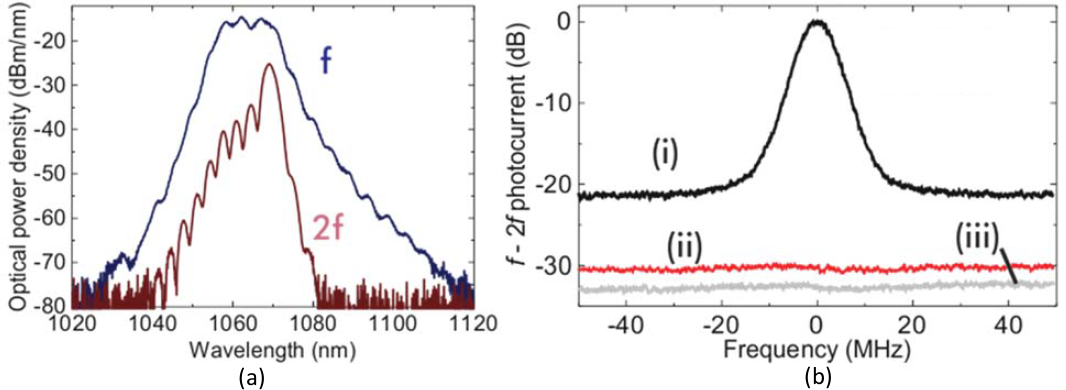
\includegraphics[width=15cm]{\FigPath/Figures/EOMCombs/EOMC_f0fromOptica.png}
	\end{center}
	\caption[Figure Title]{\textbf{Self-referencing of an EOM comb.} (a) Spectral components used for $f-2f$ self-referencing after passing through a 1070-nm optical bandpass filter: \color{red}native supercontinuum light (blue) and frequency-doubled 2140-nm supercontinuum light (red) ARE THESE LABELED CORRECTLY\color{black}. (b) Photodetected carrier-envelope offset frequency signal (black), along with a measurement of the intensity noise of the pulse train obtained by \color{red} blocking one of the paths (red) \color{black}and the photodetector noise floor (grey). \color{red}The intensity-noise measurement highlights the presence of a broad background noise floor  on the $f_0$ signal that must be the result of frequency fluctuations because it is not present when photodetecting either path alone.\color{black}}
	\label{fig:EOMC_f0}
\end{figure} 



\section{Noise in EOM Combs}

An important difference between the EOM comb scheme and other approaches for generation of frequency combs is that the repetition rate is derived from a microwave source and is multiplied directly by a factor $N$ to yield the optical frequency of the frequency-comb mode with number $N$ referenced to the seed laser (where $N=0$). Therefore, the contribution to the optical frequency noise of mode number $N$ from the microwave source scales with the mode number $N$, and the contribution to the power spectrum of frequency noise scales as $N^2$. This presents a challenge in the generation of coherent supercontinuum light, where the modes relevant for $f-2f$ self-referencing are far separated from the seed laser and $N$ is large. The factor by which the noise on the modulation tone $f_r$ is multiplied to determine its contribution to the noise on the measured carrier-envelope offset frequency is the ratio between the comb’s carrier frequency (the frequency of the seed laser) and the repetition rate: $N=f_c/f_r=$19340 for the 10 GHz comb discussed above (where $f_c=$193.4 THz for a 1550 nm seed laser). This contribution is shown in Fig. 3a, along with the contribution from the CW seed laser. The noise on $f_r$ results from technical noise on the synthesizer tone at low Fourier frequencies and approaches a white Johnson-Nyquist (thermal) phase-noise floor of -177 dBm/Hz at high Fourier frequencies. Noise in each of these regimes impacts the photodetected $f_0$ signal: low-frequency noise contributes to the linewidth of the comb modes and therefore the $f_0$ signal, while high-frequency noise contributes to a frequency-noise floor on the photodetected signal\cite{Domenico2010}. As discussed in Ref. \cite{Beha2017}, unmitigated multiplication of this noise floor by the factor $N^2=$19340$^2$ leads to a supercontinuum with optical frequency fluctuations that are large enough to prevent detection and measurement of $f_0$. 

To address this problem and enable $f-2f$ self-referencing of our comb, we pass the comb through a Fabry-Perot filter cavity whose free-spectral range is actively stabilized to the comb’s mode spacing. The filter cavity’s Lorentzian transfer function reduces the optical frequency fluctuations of the comb modes at high frequency – these fluctuations are averaged over the photon lifetime of the cavity. This enables generation of a supercontinuum with resolvable modes that is suitable for $f-2f$ self-referencing and measurement of $f_0$. 

The filter cavity used for this 10 GHz comb has a 7.5 MHz linewidth; equivalently, it has finesse of $F\sim$1333. The effect of passing the comb through the cavity is demonstrated concretely in Fig. 3b, where we compare the lineshape of a heterodyne beat between the supercontinuum and a CW laser with 1319 nm wavelength with and without the filter cavity in place. The signal-to-noise ratios for the beat with and without the filter cavity are 40 dB and 17 dB, respectively.


\begin{figure}[htpb]
	\begin{center}
		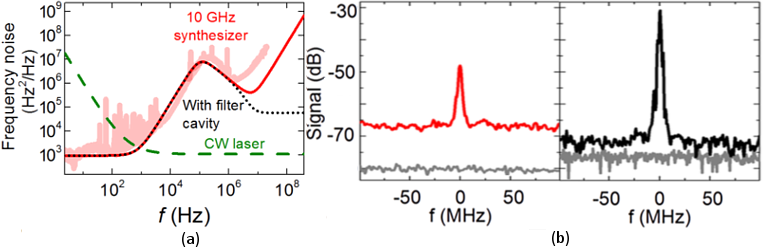
\includegraphics[width=15cm]{\FigPath/Figures/EOMCombs/EOMC_NoiseFigure_thesis.png}
	\end{center}
	\caption[Figure Title]{\textbf{Investigation of the noise properties of the EOM comb.}  (a) Contributions to the fluctuation spectrum of the carrier-envelope offset frequency: model of the input seed laser (dashed green), model of the 10 GHz synthesizer multipled by 19430$^2$ without the filter cavity (solid red, experimental data thick red), and synthesizer multiplied by 19340$^2$ and the Lorentzian filter-cavity transfer function (dotted black). (b) Comparison of the detected beats between the supercontinuum and a 1519 nm-wavelength CW laser without (red, left) and with (black, right) the Fabry-Perot filter cavity. The level of intensity noise on the supercontinuum, measured by removing the 1319 nm CW laser, is shown by the lower gray trace in each plot. Signal-to-noise ratios for the beat are 17 dB without and 40 dB with the filter cavity.}
	\label{fig:EOMC_noise}
\end{figure} 

We also explore the effect of low-frequency fluctuations in the modulation tone $f_r$ by changing the source of this tone. The $f_0$ signal shown in Fig. \ref{Fig:EOMC_f0}b is acquired with a tunable commercial synthesizer providing $f_r$. In Fig. \ref{Fig:EOMC_f0_sources} we show the detected $f_0$ signal with a dielectric-resonator oscillator and a sapphire oscillator providing $f_r$; these sources have less low-frequency noise, and the effect of this lower noise is readily apparent in the reduced linewidth of the $f_0$ signal.



\begin{figure}[htpb]
	\begin{center}
		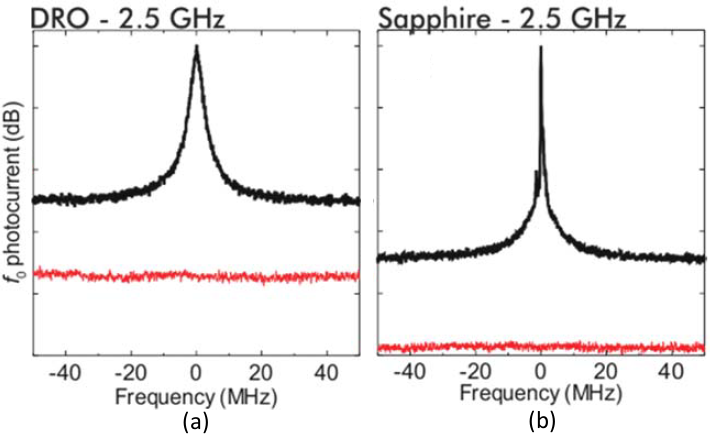
\includegraphics[width=10cm]{\FigPath/Figures/EOMCombs/EOMC_f0_diffosc_thesis.png}
	\end{center}
	\caption[Figure Title]{\textbf{Photodetected carrier-envelope-offset frequency signal with different sources for $f_r$.} (a) The $f_0$ beat resulting from a dieletric-resonator oscillator source for the modulation frequency. (b) Ibid with a sapphire oscillator as the source for $f_r$, which has lower noise than both the tunable commerical synthesizer and the DRO. The reduction in linewidth associated with the change in the source for $f_r$ shows the effect of low-Fourier-frequency noise of $f_r$ on the frequency-noise characteristics of the EOM comb. }
	\label{fig:EOMC_f0_sources}
\end{figure} 



